\documentclass{article}
\usepackage[utf8]{inputenc}
\usepackage{amsmath}
\usepackage{pdfpages}
\usepackage{booktabs}
\usepackage{hyperref}
\usepackage{enumitem}
\usepackage{url}
\usepackage{endnotes}
\usepackage[utf8]{inputenc}
\usepackage{graphicx}
\usepackage{subcaption}
\graphicspath{ {figures/} }
\usepackage{array}

\title{Intersection Pedestrian Detection and Warning System (PDWS) \\ System Concepts and Architecture}
\author{Yingying Chen & Zi'an Chen & Bingyi Fan \\ University of California, Berkeley}
\date{March 2019}

\begin{document}

\maketitle
\newpage
\tableofcontents
\listoffigures
\newpage
\section{Introduction}
Pedestrian safety has been a top priority in traffic management and control. The potentials of using intelligent transportation systems (ITS) technologies in the improvement of pedestrian safety at roadway intersections are great. 

Previous research work has shown that pedestrians are particularly vulnerable in traffic. On average, a pedestrian was killed every 2 hours and injured every 8 minutes in traffic crashes in 2013 according to National Highway Traffic Safety Administration. In 2013, pedestrian deaths accounted for 14 percent of all traffic fatalities in motor vehicle traffic crashes. 
\endnote{Traffic Safety Facts: Data of 2013, NHTSA, Mar. 2015, available at \url{https://crashstats.nhtsa.dot.gov/Api/Public/ViewPublication/812124}}
The final report of the IDS project at California PATH has pointed out that a significant amount of future research should be devoted to the incorporation of an ITS sub-system for the improvement of pedestrian safety.
\endnote{Jim Misener, et al.\textit{ California Intersection Decision Support: A Systems Approach to Achieve Nationally Interoperable Solutions II.} 2007, p. 29}

Additionally, we believe that existing control methods are insufficient to protect the pedestrians from accidents with vehicles at uncontrolled intersections and at mid-block crosswalks. In those kinds of intersections, motor vehicles often fail to yield the right-of-way to crossing pedestrians, and pedestrians are also hard to be spotted at night. Thus, we believe that an adequate ITS technology for pedestrian safety is urgently needed at those locations. Mr. Bingyi Fan, one of the authors, has personally survived a hit-and-run accident at an uncontrolled intersection in South Lake Tahoe, California, attested to the necessity of such a system and contributed his insight into its design.

Our project builds upon the achievements of the IDS project and focuses on pedestrian safety and the contributions are:
\begin{itemize}
    \item to design a sensing, communication, and warning system for a designated intersection;
    \item to improve pedestrian safety by using accurate detection technologies and visible signage that are provided to both the vehicles and the pedestrians;
    \item to explore the possibility of mass deployment of this system.
\end{itemize}


\subsection{The Intersection}
As shown in Figure \ref{fig:intersect}, the designated study intersection is at Shattuck Ave. \& Virginia St., in Berkeley, California. 

\begin{figure}
    \centering
    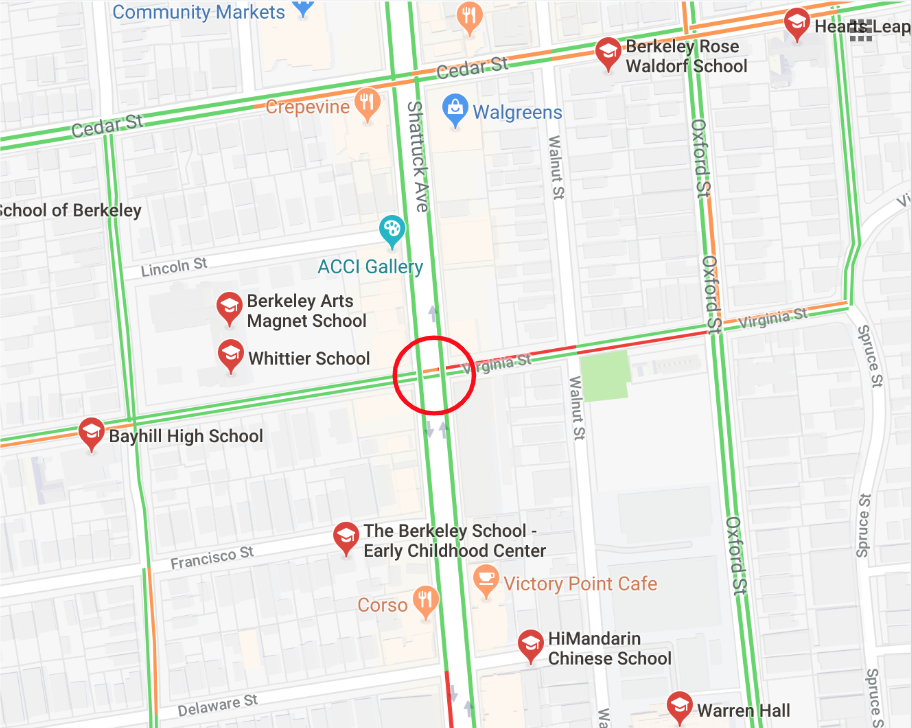
\includegraphics[width=12cm]{intersection1.png}
    \caption{Intersection of Shattuck Ave. \& Virginia St. in Berkeley}
    \label{fig:intersect}
\end{figure}

\begin{figure}
    \centering
    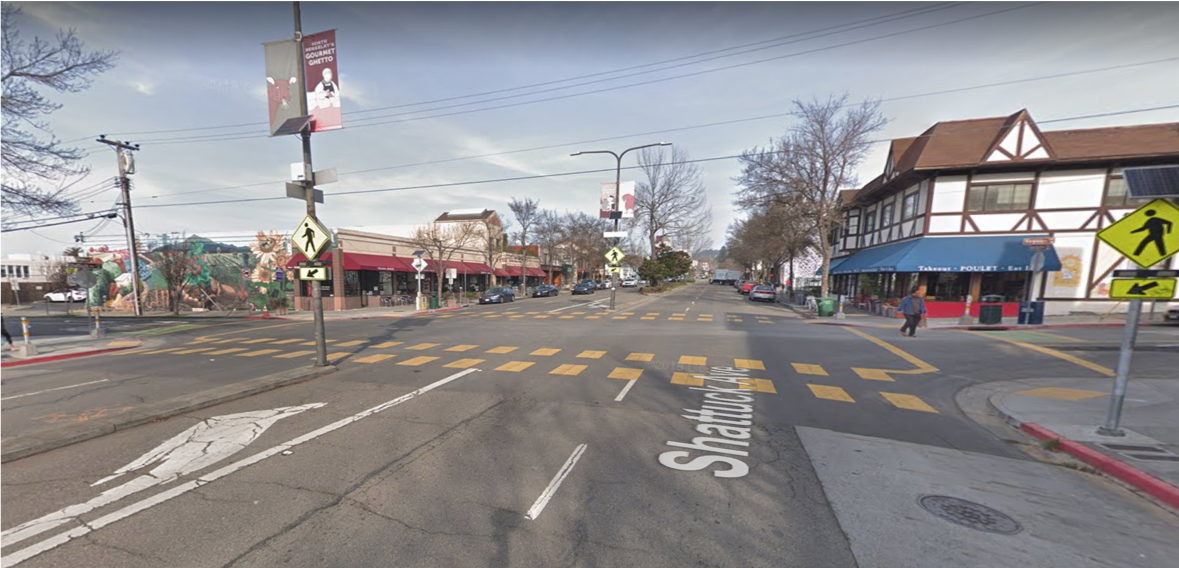
\includegraphics[width=12cm]{int_photo.png}
    \caption{Picture of the Intersection}
    \label{fig:intersect_pic}
\end{figure}

\subsection{Roadway Specifics}
Shattuck Ave. is the major north to south artillery with 2 through lanes and 1 dedicated left-turn lane in each direction.

Virginia St. is the minor east to west roadway with 1 lane in each direction.

There are crosswalks on all four sides of the intersection.

Figure \ref{fig:intersect_pic} shows the layout of the intersection and some of the equipment at the intersection that will be discussion in the next subsection. As labeled in red dots in the figure, there are more than eight schools in the map area. There are also lots of restaurants and grocery stores around the area. As a school zone and a pedestrian-heavy intersection, this section is worth studying.

\subsection{Existing Control Equipment}
Currently, there are stop signs on Virginia Ave., but traffic on Shattuck Ave. is not controlled.

A set of pedestrian crossing warning signs exist on Shattuck Ave., which, once manually activated by a crossing pedestrian by pushing a button, will flash yellow LED lights for 20 seconds to warn the vehicles. However, from our \textit{in situ} observations , pedestrians often forget to turn on the flashing lights. Besides, they are prone to be ignored by the drivers. 

\section{The Sensing System}
We chose to implement FLIR TrafiSense Thermal Imaging Traffic Sensors for the detection system, which will be discussed further in details in the following sections.

\subsection{FLIR TrafiSense Thermal Imaging Traffic Sensors}
FLIR produces multiple models of the TrafiSense sensors. Figure \ref{fig:FLIR_spec} shows the specifications of different models. Among them, model ETH/BPL 345 is suitable for the use of this project as it provides all the functionalists that is required to meet our need and an appropriate detection range of up to 160 ft.

\begin{figure}
    \centering
    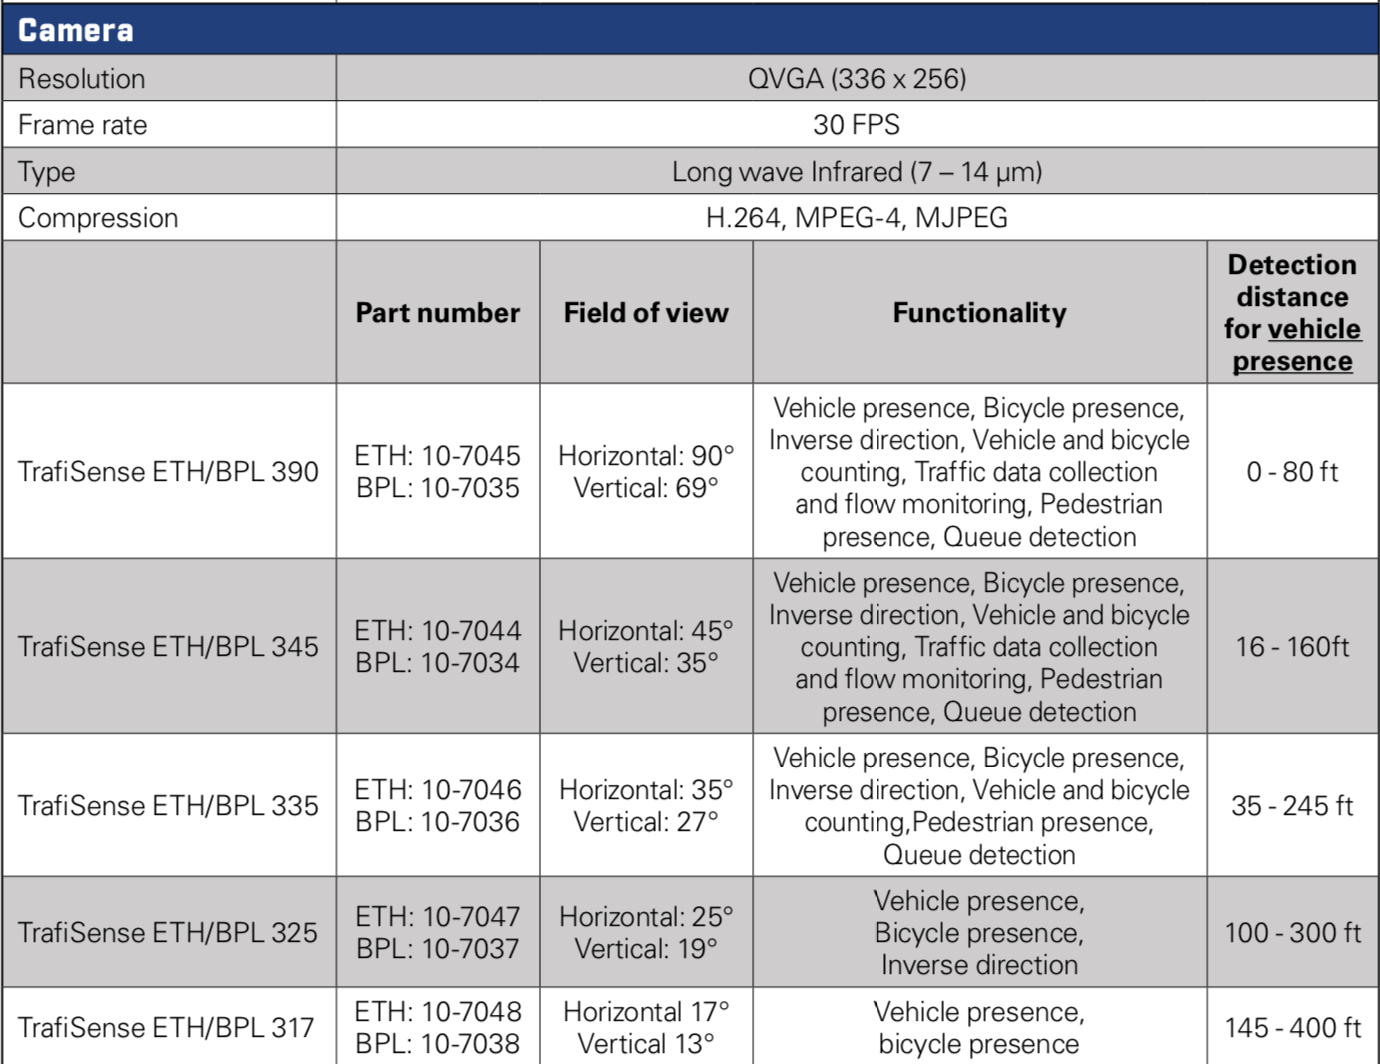
\includegraphics[width=12cm]{FLIR_spec.png}
    \caption{Specifications of the FLIR Sensors}
    \label{fig:FLIR_spec}
\end{figure}

\begin{figure}
    \centering
    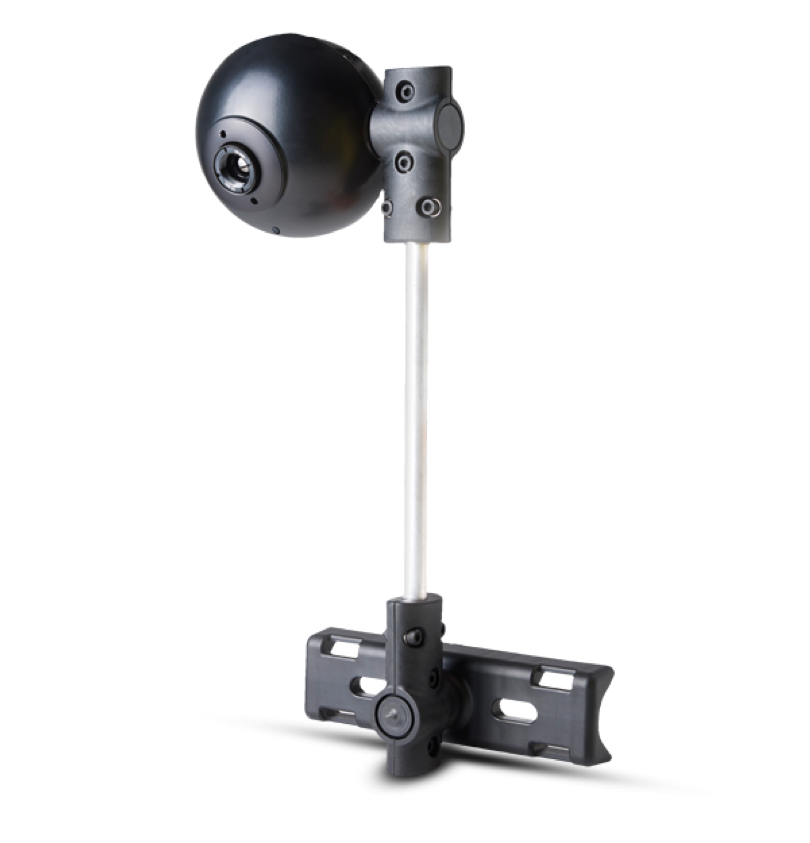
\includegraphics[width=6cm]{FLIR.png}
    \caption{FLIR TrafiSense Thermal Imaging Traffic Sensor}
    \label{fig:FLIR}
\end{figure}

In this section, we will discuss the advantages of the FLIR TrafiSense Sensor. Please see Figure \ref{fig:FLIR} for an image of the FLIR TrafiSense Thermal Imaging Traffic Sensor.
\begin{itemize}
\item The FLIR TrafiSense is a high-resolution thermal imaging sensor, which enables it to be operational during day time as well as night time and even in inclement weather conditions.
\item As shown in Figure \ref{fig:FLIR_zone}, one of its greatest advantages is that it is able to focus on defined zones.
\item Besides, it is also able to distinguish between vehicles, pedestrians, and bicycles, as shown in Figure \ref{fig:FLIR_thermal}.
\item In addition, the direction a vehicle or pedestrian heading to could also be predicted by the sensor. Figure \ref{fig:FLIR_thermal} below shows on-crossing pedestrian detection of the sensing system.
\item The detector is programmable to have more functions as well.
\end{itemize}

\begin{figure}
    \centering
    \begin{subfigure}[b]{0.5\textwidth}
        \centering
        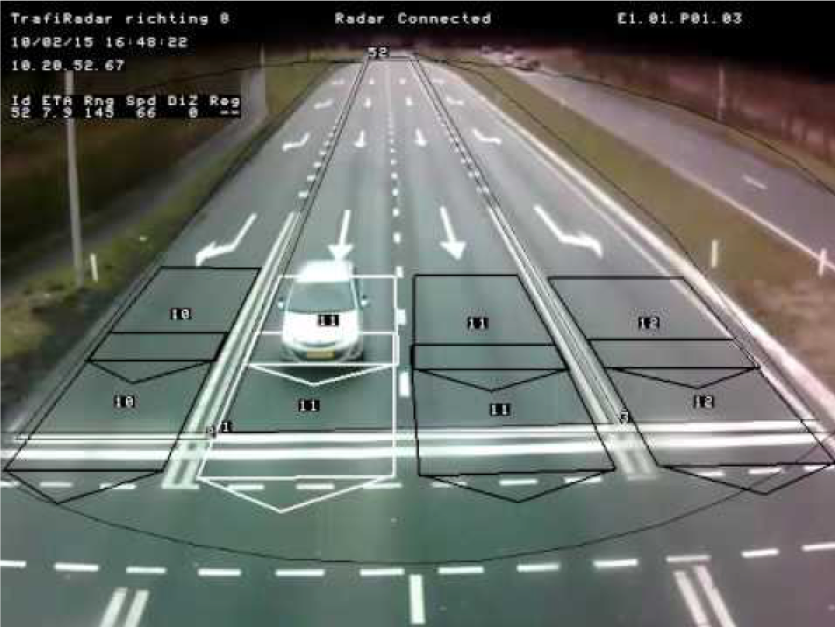
\includegraphics[width=\textwidth]{FLIR_zone.png}
        \caption{Vehicle Zone Detection}
        \label{fig:FLIR_zone}
    \end{subfigure}%
    \begin{subfigure}[b]{0.5\textwidth}
        \centering
        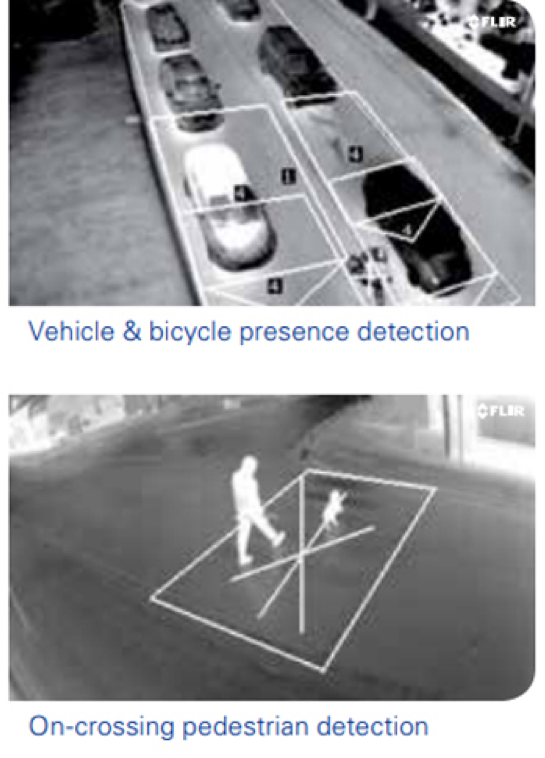
\includegraphics[width=\textwidth]{FLIR_thermal.png}
        \caption{Pedestrian Movement Detection}
        \label{fig:FLIR_thermal}
    \end{subfigure}
    \caption{Demonstration of FLIR Sensor Functionalists}
\end{figure}

\subsection{Other Components}
Other hardware components of the sensing system includes:
\begin{itemize}
    \item FLIR XStream Computing Box: The computing box collects data from the sensor and sends commands.
    \item Computer Unit: The computer unit processes data and controls and whole system, which could be placed either on roadside or in a Traffic Management Center.
\end{itemize}

\subsection{Placement of FLIR Sensors}
In this section, we will discuss the placement of the FLIR sensors around the intersection. 

To get a full coverage of the intersection, including the nearby roadway segments and all four crosswalks, the project team has decided to place two FLIR TrafiSense Model ETH/BPL 345 sensors at the study site, with one at the north-west corner of the intersection, and the other at the south-east corner. As shown in Figure \ref{fig:sensor_position}, the two sensors are expected to cover all four crosswalks and street corners as well as lanes from each direction, including the three lanes of Shattuck Avenue. Both of the sensors will be placed at 20 feet height according to specifications and ranges of the FLIR detectors. Blue and red zones for different levels of warning methodologies will be programmed into the control software of the FLIR sensors for detection. Specifics of the blue and red zones such as positions and dimensions will be discussed in details in the section of timing and control algorithms.

The placement plan is tentative because further experiments such as in-house experiments that simulate real-world scenarios need to be conducted to test and verify the placement of the sensing system and to calibrate the configurations of the equipment. After that, field experiment on the intersection could probably be done as well if needed.

\begin{figure}
    \centering
    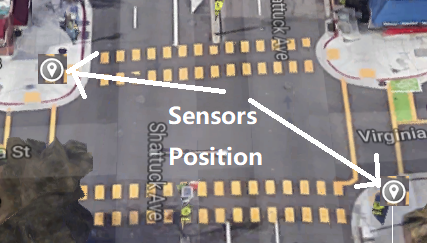
\includegraphics[width=12cm]{sensor_pos.png}
    \caption{Sensor Position}
    \label{fig:sensor_position}
\end{figure}

\subsection{Comparisons between FLIR and Traditional Equipment}
Advantages and disadvantages of FLIR sensor versus traditional traffic cameras or detectors are as follows:

\begin{itemize}

    \item FLIR TrafiSense Thermal Imaging Traffic sensor:
    \begin{itemize}
        \item Pros: As discussed earlier in section 2.1, this particular thermal imaging sensor is intelligent and multi-functional. 
        \item Cons: Despite all of its advantages, this type of state-of-the-art sensor is expensive. The negotiated wholesale price for a bulk order of $>20$ cameras is approximately \$3,000 each, and the retail price is even higher.
    \end{itemize}
    
    \item Traditional traffic cameras/sensors:
    \begin{itemize}
        \item Pros: As compared to the FLIR TrafiSense sensor, traditional cameras are at a relatively low cost.
        \item Cons: Because the traditional ones are not as intelligent as the chosen sensor, to enable the functions required for the project, a team of back-end software developers need to be hired to implement designated functions, which leads to relatively high cost in the long run.
    \end{itemize}
    
\end{itemize}


\section{Timing and Control Algorithms}
\subsection{Procedure of Conflict Detection}
The following procedure is developed to determine if there is an active conflict between the (intended) route of movement the pedestrian and the (intended) route of movement of the pedestrian. If multiple vehicles and/or pedestrians are present at the same time, multiple procedures will be called and the most restrictive result will be returned (with OR logical).

The conflict diagrams provided in Figure \ref{fig:condlict} demonstrates that vehicle in the left lane conflicts with pedestrians crossing on the left or in the near front; vehicle in the center lane conflicts with pedestrians crossing in the near and far front; and vehicle in the right lane conflicts with pedestrians crossing in the near and far front and on the right. The red boxes represent conflict and the green boxes represent no conflict.

The inputs to this procedure are the current lane of the approaching vehicle and the route of movement of the pedestrian. If the pedestrian is already on a crosswalk, the route can easily be determined by the location of the crosswalk; if the pedestrian is starting crossing at a corner, his/her intended direction of moving, supplied by the FLIR sensors, will be used.

\begin{verbatim}
Procedure ConflictDetection(sensor input)
    Return True If (
        ped crossing in near front OR on the left AND veh in left lane OR 
        ped crossing in front AND veh in center lane OR
        ped crossing in front or on the right If veh in right lane
        )
\end{verbatim}
\begin{figure}
    \centering
    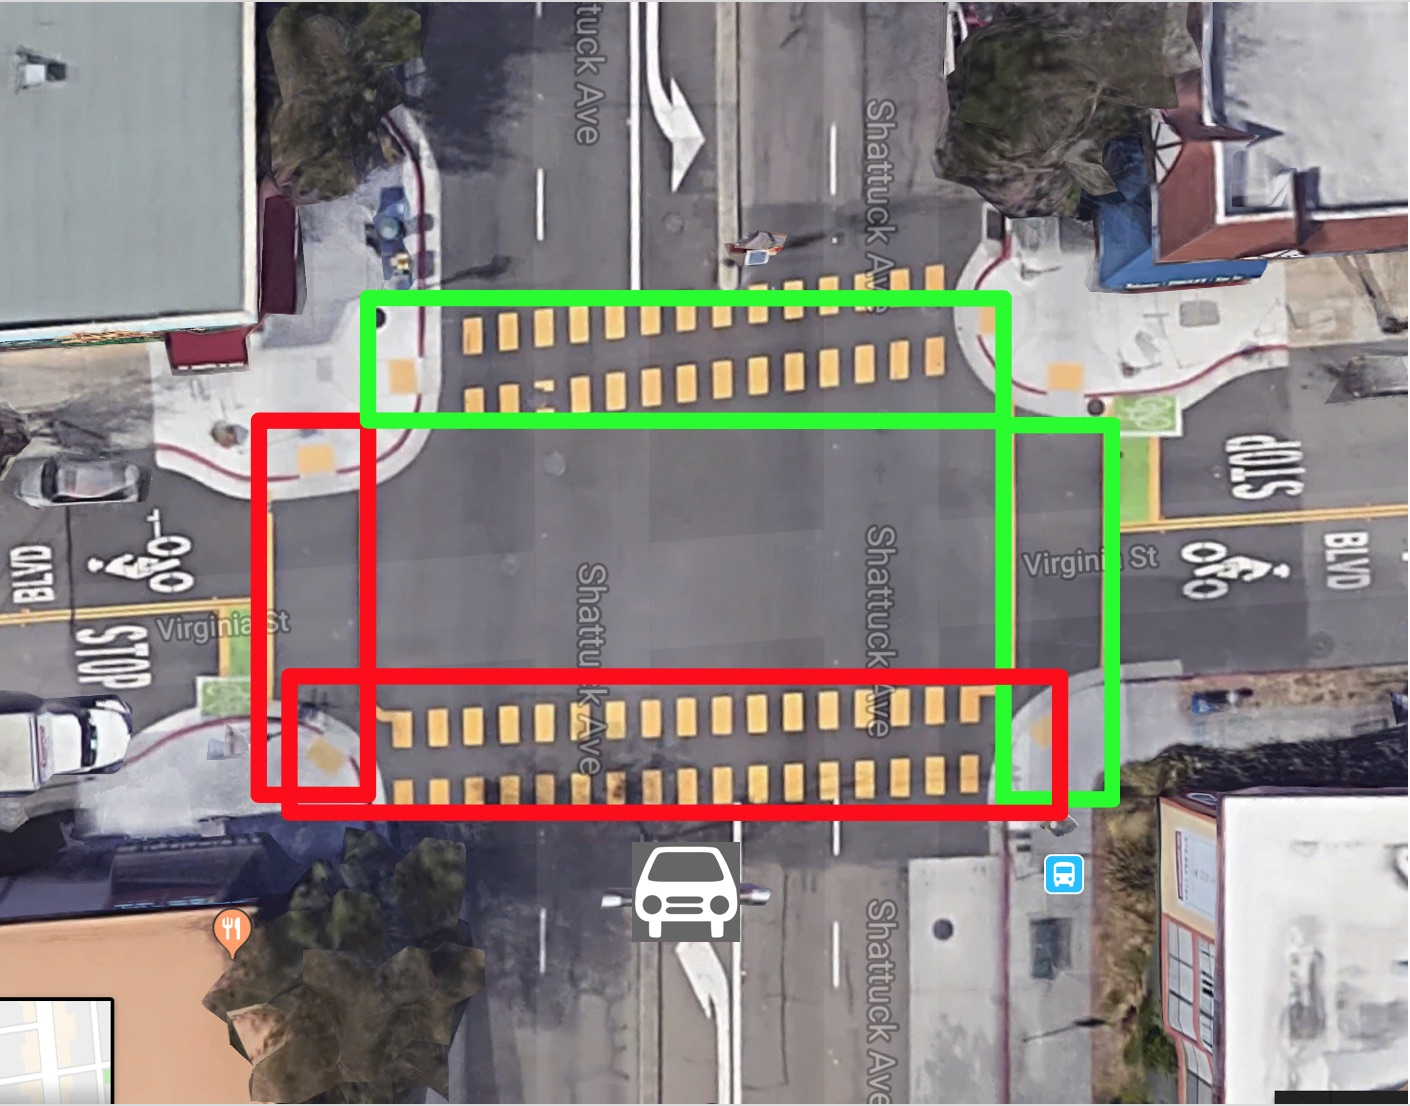
\includegraphics[width=7cm]{left.jpg}
    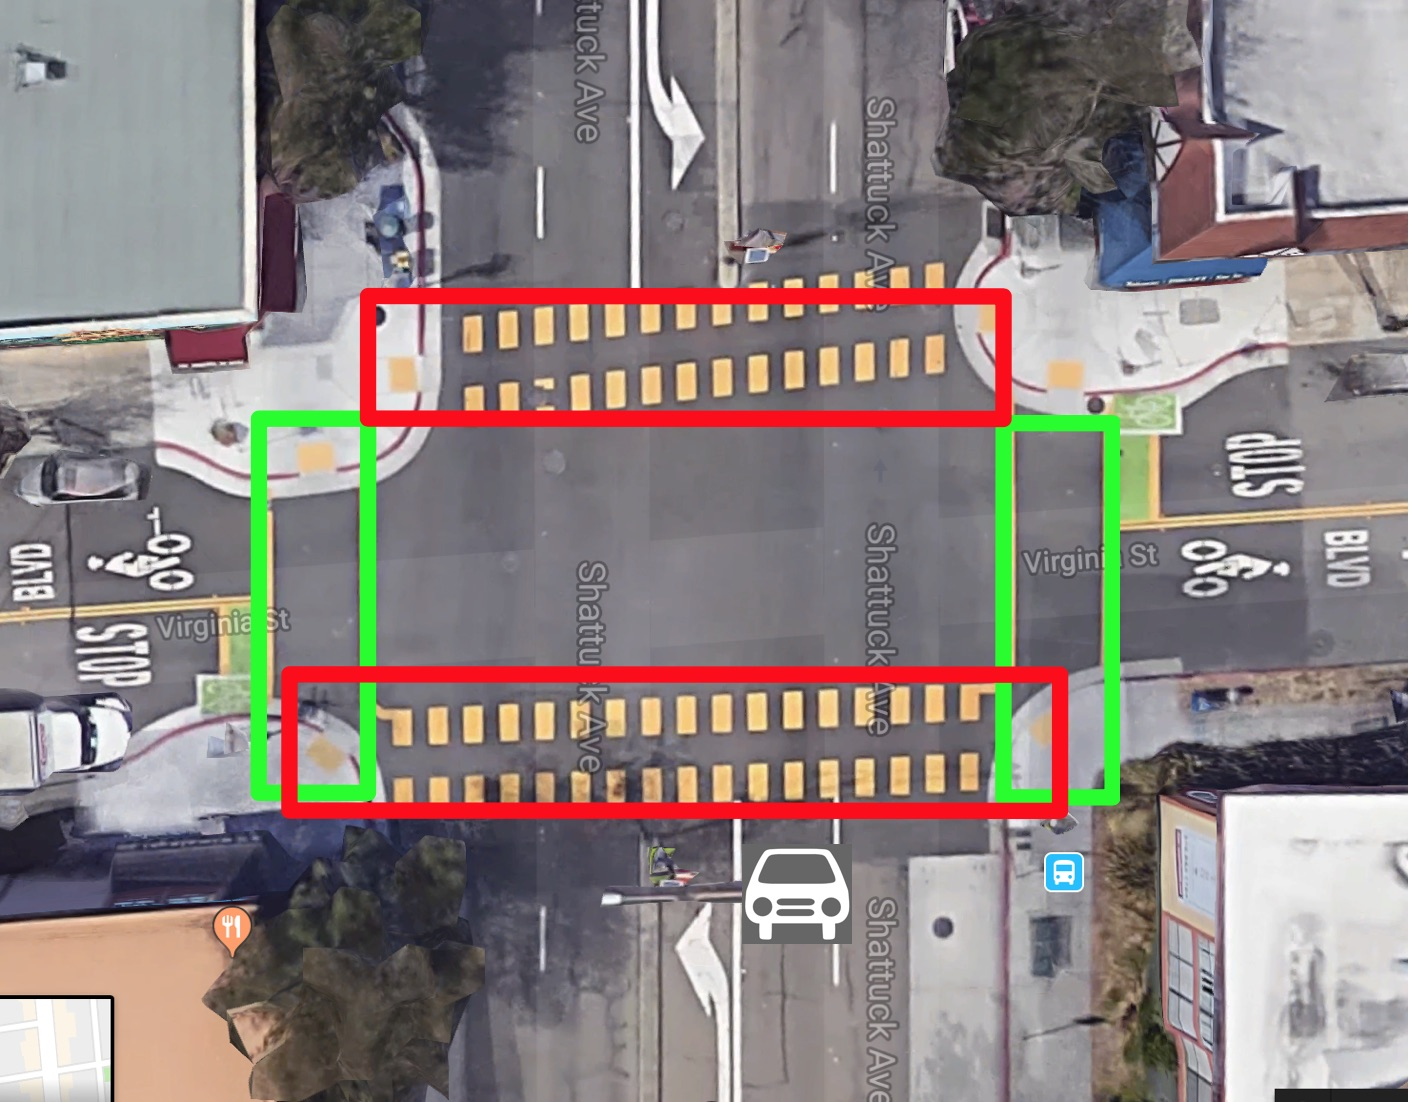
\includegraphics[width=7cm]{center.jpg}
    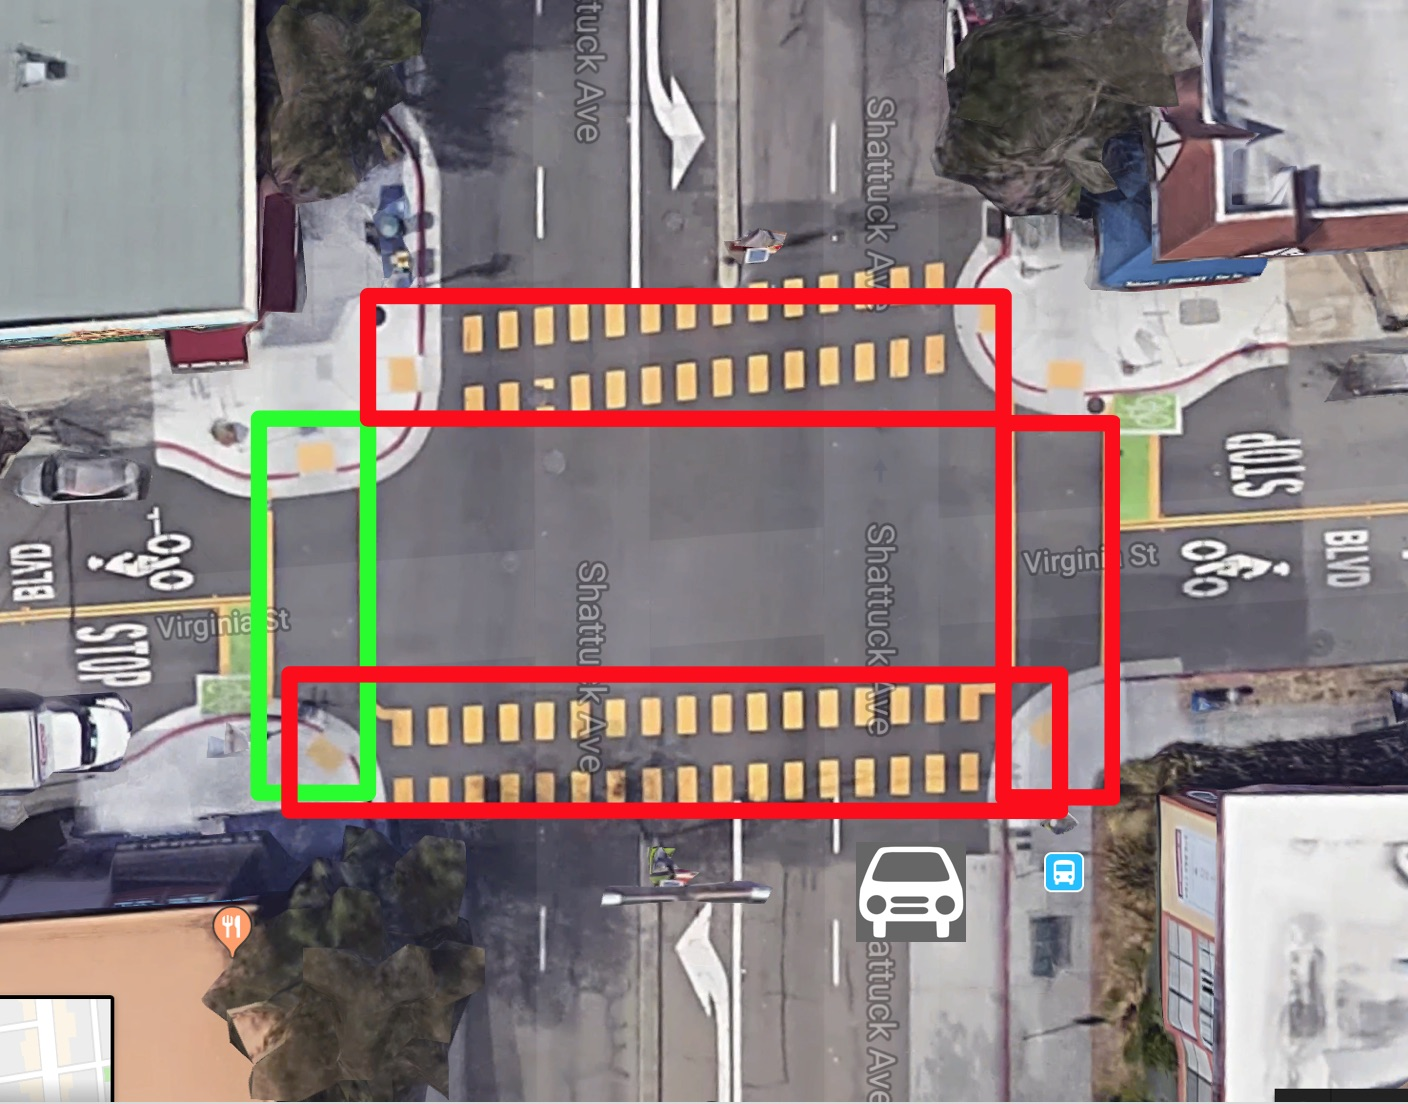
\includegraphics[width=7cm]{right.jpg}
    \caption{Conflict Diagrams}
    \label{fig:condlict}
\end{figure}

% \begin{figure}
%     \centering
%     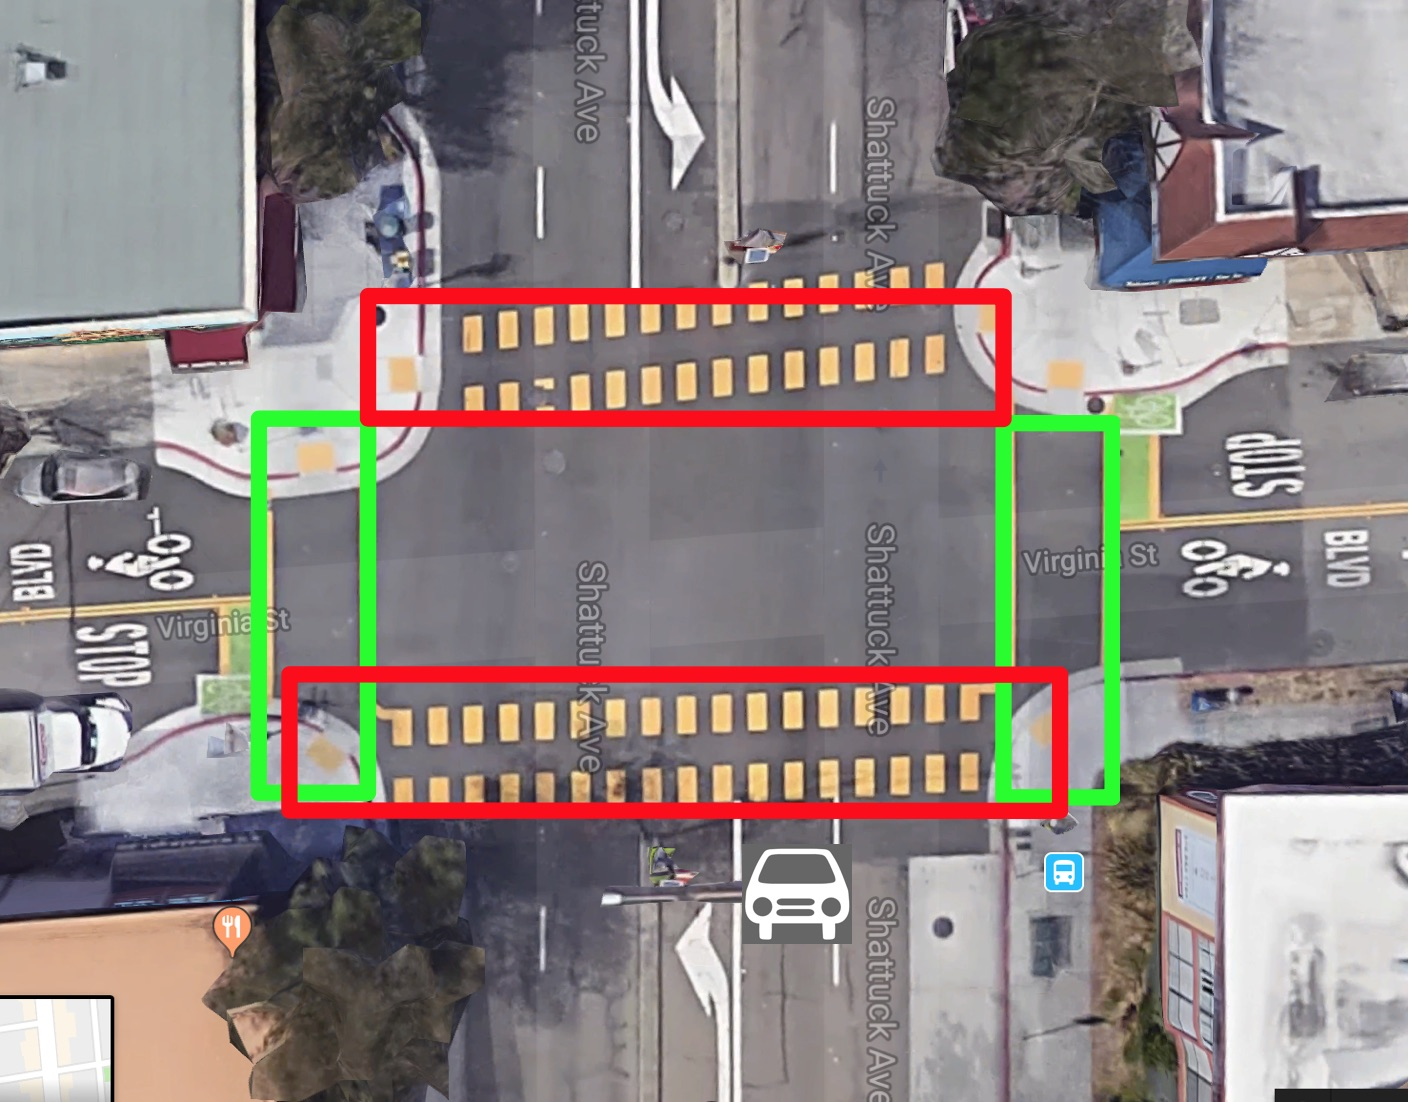
\includegraphics[width=10cm]{center.jpg}
%     \caption{Conflict Diagram: Vehicle in the center lane: conflict with peds crossing in the near and far front}
% \end{figure}

% \begin{figure}
%     \centering
%     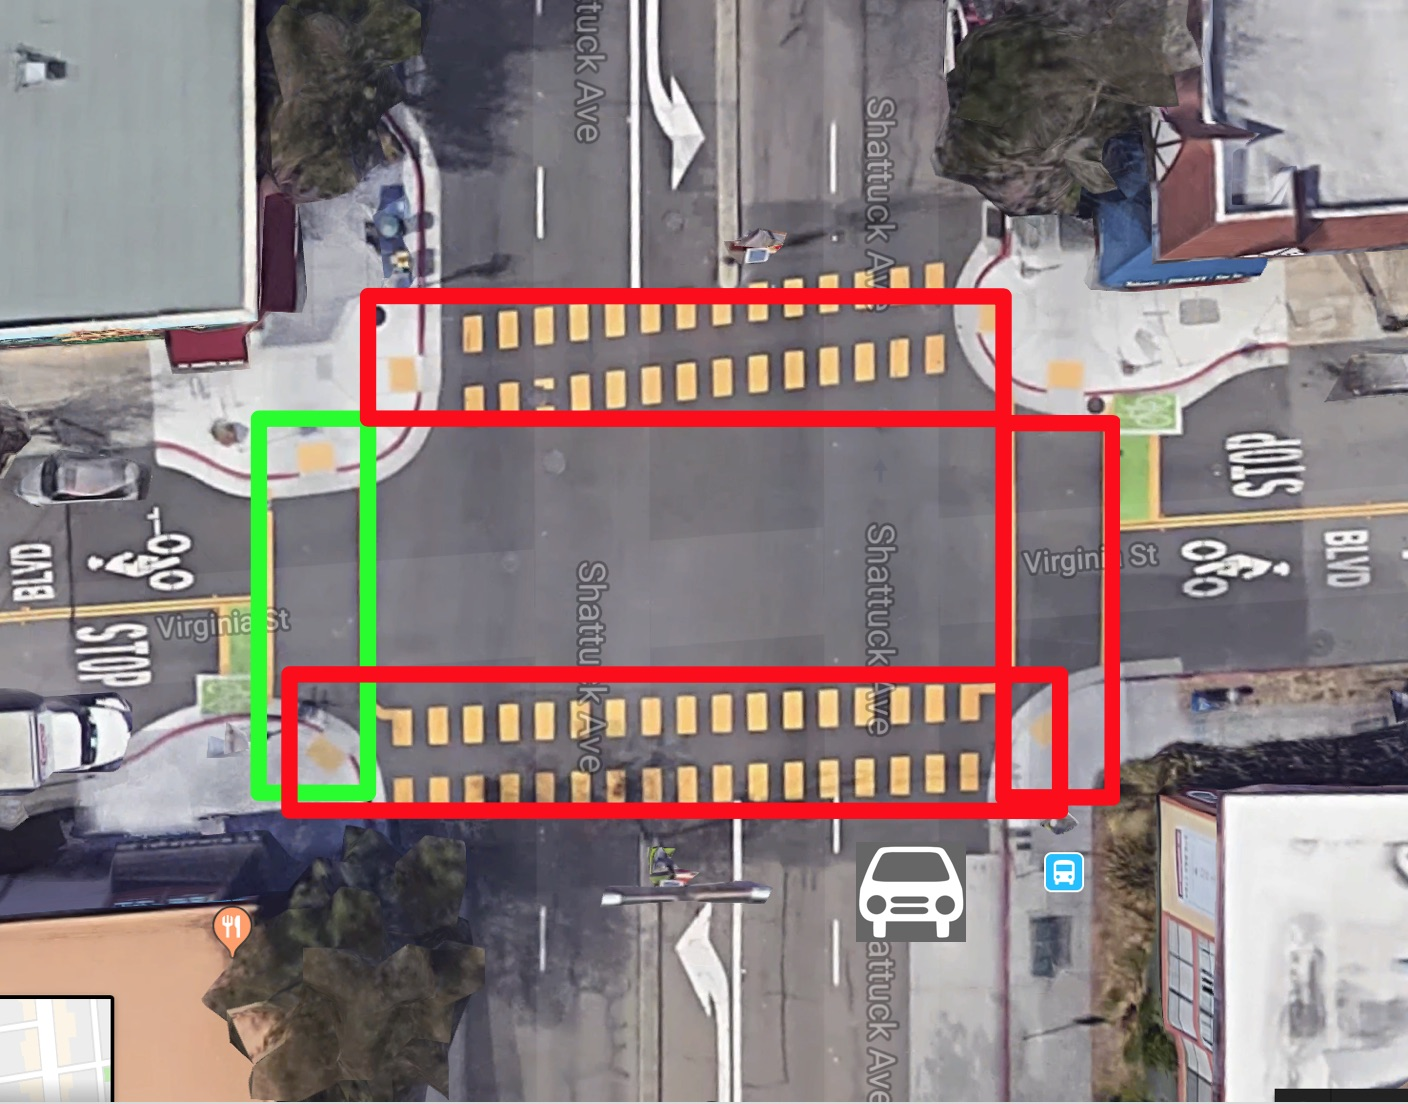
\includegraphics[width=10cm]{right.jpg}
%     \caption{Conflict Diagram: Vehicle in the right lane: conflict with peds crossing in the near and far front and on the right}
% \end{figure}

\subsection{Control of Warning Signs for Vehicles and Pedestrians}
This is the main algorithm that will be used to control the warning signs that are designed to provide warnings to the vehicles and the pedestrians if a danger of accident is detected. It relies on the \texttt{ConflictDetection} procedure to determine if there is a conflict and determine the location of the conflict.
\begin{verbatim}
While ped in crossing
    While veh in blue OR red zones do
        If Conflict then
            vehWarning YELLOW
            pedWarning ON
            If speed > 20 then
                vehWarning YELLOW, FLASHING LOW
            End If
            If speed > 30 then
                vehWarning RED, FLASHING LOW
            End If
            If speed > 10 and veh in red zone do
                vehWarning RED, FLASHING HIGH
                pedWarning FLASHING
                (take picture)
            End If
        End If
    End While
End While
\end{verbatim}

To summarize, the algorithm will control the warning signs depending on whether the vehicle is in the red or blue zone, shown in Figure \ref{fig:zones} and explained in detail in the next section, and the vehicle's speed. The warning sign for vehicles have five possible status: all light off, yellow light on, red light on, flashing with low frequency and flashing with high frequency. A vehicle being in the red zone and/or with a high speed is considered more dangerous and different status of the signage will be activated according to the level of perceived threat.

There is also a warning sign intended for the pedestrians. In the most dangerous situation, the sign will be activated to warn the pedestrians to stop walking in case the vehicle fails to stop and yield.

\subsection{Warning Zones}
\subsubsection{Definition of Red and Blue Zones}
We designated two zones on the road segment approaching the intersection. The red zone is the area closer to the stop line, in which an approaching vehicle posts a high threat to the pedestrian, and the blue zone is the area farther away, in which an approaching vehicle posts a moderate threat to the pedestrian. The ranges of the red zone and the blue zone are determined by the assumed stop distance of a typical vehicle.

The blue zone should cover a distance at which a vehicle is able to normally stop to yield to a crossing pedestrian, and the red zone should cover a distance at which a vehicle is able to apply emergency break, if necessary, to yield to a crossing pedestrian. 

\begin{figure}
\centering
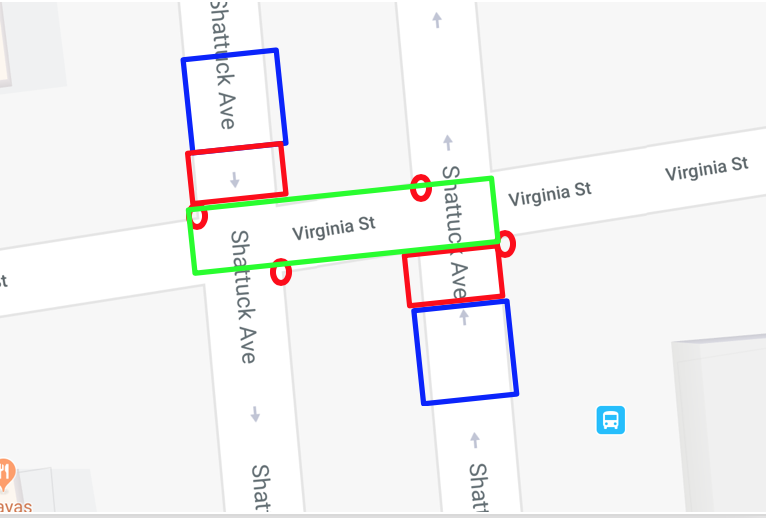
\includegraphics[width=11cm]{zones.png}
\caption{Red and Blue Zones}
\label{fig:zones}
\end{figure}

\subsubsection{Calculation of Zone Ranges}
The ranges of zones are to be calculated with formulas of physics, with parameters to be adjusted with the specifics of vehicles and roadways.

The formula that tells the distance it takes for a moving vehicle to come to a complete stop is
\begin{equation}
    \displaystyle d = \frac{v^2}{2\mu g}
\end{equation}

where
\begin{itemize}[noitemsep]
    \item $d$ = stopping distance (m)
    \item $v$ = initial velocity (m/s)
    \item $\mu$ = coefficient of friction, assumed to be 0.81\endnote{Serway, Raymond A. and Robert J. Beichner. \textit{Physics for Scientists and Engineers with Modern Physics}, 5th edition. New York: Saunders, 133.} for rubber on dry concrete 
    \item $g$ = gravitational constant, $9.81 m/s^2$
\end{itemize}

For the total stopping distance, we also have to consider the reaction time of the driver.

\begin{equation}
d_{\text{total}} = d_{\text{stopping}} + d_{\text{reaction}} = d_{\text{stopping}} + vt
\end{equation}

where 
\begin{itemize}[noitemsep]
    \item $d_{\text{reaction}}$ = $d$ obtained in (1)
    \item $v$ = initial velocity (m/s)
    \item $t$ = reaction time (s)
\end{itemize}

We assume that, for vehicles in the blue zone, their drivers have a normal reaction time of 2.3 s \endnote{Driver Reaction Time in Crash Avoidance Research: Validation of A Driving Simulator Study on A Test Track, available at \url{ https://copradar.com/redlight/factors/IEA2000_ABS51.pdf}}, and, for vehicles in the red zone, their drivers have an emergency reaction time of 1.5 s \endnote{Stopping Distances: Speed and Braking, Driving Safely and to the Road Conditions. Transport and Motoring, Queensland Government, 14 Nov. 2016, available at \url{http://www.qld.gov.au/transport/safety/road-safety/driving-safely/stopping-distances}}. We assumed that the initial velocity of a vehicle entering the blue zone to be 30 mph, at which velocity the yellow warning sign will be triggered with high frequency. We also assumed that the initial velocity of a vehicle entering the red zone to be 20 mph, at which velocity the red warning sign will be triggered with flashing.

After calculation and approximation, we determined that, with all the assumptions stated above, the range of the red zone is 0 - 10 m before the stop line and the range of the blue zone is 10 - 30 m before the stop line.

We did consider that the Northside of Berkeley is a hilly area and the grade of the roadway may cause the vehicle to have a longer or smaller stopping distance. However, after a field visit, we determined that the segment of Shattuck Ave. at Virgnia Ave. is relatively flat and the influence of grade is negligible. (East-West oriented roadways, like Virginia Ave., Cedar St., etc., are more hilly and the grade may affect the stopping distance there.)

\section{The Signage System}
\subsection{Design of Warning Signs}
We designed the customized warning signs for our system that can be controlled by the algorithm in the previous section. 

The graphics in Figure \ref{fig:warning_signs} are a representation of the design of the signs. In addition, yellow and/or red LED lights should be installed above both signs according to the algorithmic design. 

For the warning sign for vehicles, the blackened area with the word "front" in it represents a small LED screen, which can display the location of the crossing pedestrian relative to the vehicle. Possible words to be displayed include "left", "front" and "right".

\begin{figure}
    \centering
    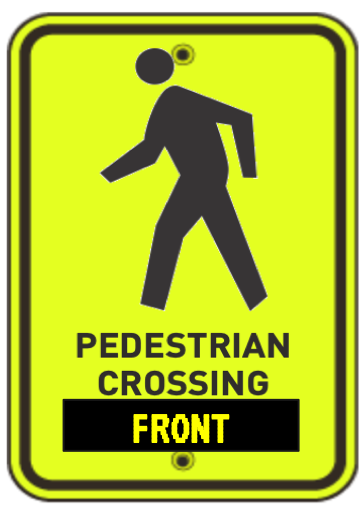
\includegraphics[width=6cm]{warn1.png}
    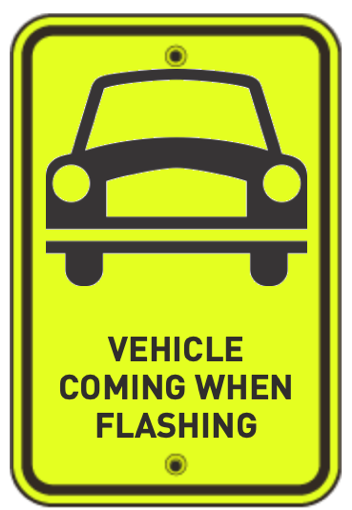
\includegraphics[width=5.8cm]{warn2.png}
    \caption{Warning Signs for Vehicles and for Pedestrians}
    \label{fig:warning_signs}
\end{figure}

Actual signs are to be manufactured according to the MUTCD \endnote{California manual on uniform traffic control devices for streets and highways (FHWA's MUTCD 2009 edition, as amended for use in California), 2012, Sacramento, CA: State of California, Business, Transportation and Housing Agency, Dept. of Trans} standards, which recommends a size of 36' x 36' for rectangular signs on a conventional multi-lane roadway.

\begin{figure}
    \centering
    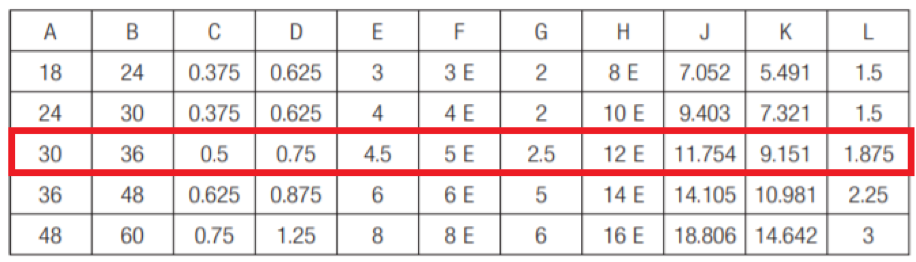
\includegraphics[width=12cm]{mutcd.png}
    \caption{Excerpt from the MUTCD Standards}
    \label{fig:mutcd}
\end{figure}

\subsection{Positions of Warning Signs}

The warning signs are placed on the right hand side of the roadway, at each entrance of the intersection as well as the far middle corner. The height of signs are 7 feet, measured vertically from the bottom of the sign to the sidewalk according to the MUTCD standard. 

\subsection{In Vehicle Warning Device}

The In Vehicle Warning Device is achieved by Wireless infrastructure used to communicate between vehicles and intersection called Dedicated Short-Range Communications (DSRC). Vehicles installed this function will have a safer driving experience by receiving direct warning messages when necessary.

Sensors sensing a incoming vehicle that may be in conflict pedestrians will send signals to the vehicle. The signals will be analyzed and converted to messages telling drivers to yield to pedestrians. The messages will be displayed on the screen of vehicles along with warning sound at the frequency of 2 beeps per second.

\begin{figure}
    \centering
    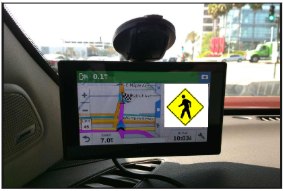
\includegraphics[width=6cm]{in_car_warning.png}
    \caption{In-Vehicle Warning Message}
    \label{fig:veh_warning}
\end{figure}

\section{Concluding Remarks}

In this project, the team designed a pedestrian detection and warning system to be deployed at an experiment road intersection in Berkeley, California. The system makes use of start-of-the-art intelligent transportation technologies, including thermal imaging traffic sensors, computing algorithms and signage systems. The technology based IDS approach addresses pedestrian safety, which is an issue of great importance in intersection dynamics as described by Jim in the IDS Final Report.

Although we designed the system as carefully as we could, for deployment it must go through a series of in-house experiments, revisions and calibrations. Design specifics of the systems are subject to change.

The current goal of the project is to deploy a prototype system to the Shattuck at Virginia intersection. If the prototype proves to be functional, we would revise the design according to the data collected and aims to make the system more standardized, generic and adaptable that can be mass-deployed in a wide range to improve pedestrian safety on our nation's roadways.

\newpage
\theendnotes




% \bibliographystyle{plain}
% \bibliography{references}
    
%     https://crashstats.nhtsa.dot.gov/Api/Public/ViewPublication/812124
%     
%     https://mutcd.fhwa.dot.gov/htm/2009/part2/part2c.htm#section2C50

\end{document}

